\documentclass[a4paper]{article}

\usepackage{graphicx}
\usepackage{amsmath,amssymb}
\usepackage{minted}
\usepackage{multirow}
\usepackage{float}
\usepackage{todonotes}
\usepackage{forest}
\usepackage{xstring}
\usepackage{xcolor}
\usepackage[most]{tcolorbox}
\usepackage{xparse}
\usepackage{natbib}

\usetikzlibrary{graphs,graphdrawing}
\usegdlibrary{layered}

% for external graphviz
\input{/home/donkarlo/Dropbox/repo/nd_ai_project/src/nd_ai/knoweldge_representation/language/formal/computer/programming/tex/latex/code_clips/external_graphviz.tex}

% for tags
\input{/home/donkarlo/Dropbox/repo/nd_ai_project/src/nd_ai/knoweldge_representation/language/formal/computer/programming/tex/latex/parts/control_sequence/kind/semtag/semtag.tex}

% for links
\input{/home/donkarlo/Dropbox/repo/nd_ai_project/src/nd_ai/knoweldge_representation/language/formal/computer/programming/tex/latex/code_clips/seehere.tex}

\title{Zeitadverbieren}
\date{}

\begin{document}
    \maketitle
    \begin{figure}[H]
        \centering
        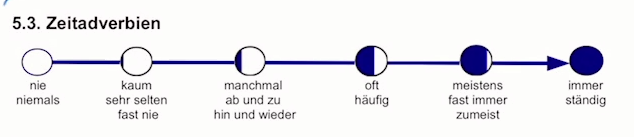
\includegraphics[width=0.9\textwidth]{zeitadverbien.png}
    \end{figure}
        
        \section{nie / niemals}
            
            \textbf{Bedeutung:} never
            
            \begin{itemize}
                \item Ich rauche nie. -- I never smoke.
                \item Sie kommt niemals zu spät. -- She never comes late.
                \item Ich habe ihn nie gesehen. -- I have never seen him.
            \end{itemize}
        
        \section{kaum / sehr selten / fast nie}
            
            \textbf{Bedeutung:} hardly ever / very rarely / almost never
            
            \begin{itemize}
                \item Ich esse kaum Fleisch. -- I hardly ever eat meat.
                \item Er geht sehr selten ins Kino. -- He very rarely goes to the cinema.
                \item Wir sehen uns fast nie. -- We almost never see each other.
            \end{itemize}
        
        \section{manchmal / ab und zu / hin und wieder}
            
            \textbf{Bedeutung:} sometimes / now and then / occasionally
            
            \begin{itemize}
                \item Manchmal trinke ich Kaffee. -- Sometimes I drink coffee.
                \item Ab und zu gehe ich spazieren. -- Now and then I go for a walk.
                \item Hin und wieder besuche ich meine Freunde. -- Occasionally I visit my friends.
            \end{itemize}
        
        \section{oft / häufig}
            
            \textbf{Bedeutung:} often / frequently
            
            \begin{itemize}
                \item Ich lese oft deutsche Texte. -- I often read German texts.
                \item Sie hört häufig Musik. -- She frequently listens to music.
                \item Wir gehen oft zusammen einkaufen. -- We often go shopping together.
            \end{itemize}
        
        \section{meistens / fast immer / zumeist}
            
            \textbf{Bedeutung:} mostly / almost always / usually
            
            \begin{itemize}
                \item Meistens stehe ich früh auf. -- I mostly get up early.
                \item Er ist fast immer pünktlich. -- He is almost always on time.
                \item Zumeist arbeite ich am Vormittag. -- Usually I work in the morning.
            \end{itemize}
        
        \section{immer / ständig}
            
            \textbf{Bedeutung:} always / constantly
            
            \begin{itemize}
                \item Ich denke immer an meine Prüfung. -- I always think about my exam.
                \item Sie ist immer freundlich. -- She is always friendly.
                \item Er schaut ständig auf sein Handy. -- He constantly looks at his phone.
            \end{itemize}
%            \bibliographystyle{plainnat}
%            \bibliography{/home/donkarlo/Dropbox/repo/nd_shared_research/bibliography/bibliography.bib}
\end{document}